%% FSE (CS-5187 Term Project) research paper. Requirements from the CFP (https://conf.researchr.org/home/fse-2026, checked 2026-09-30):
%%   * \documentclass[acmsmall,screen,review,anonymous]{acmart}; single column
%%   * 12 pages of text and figures + references not counted (course limit, paper.conf)
%%   * double-anonymous: no names, no identifying URLs, third-person
%%     self-citation, no acknowledgments at submission
%%   * "Data Availability" section after the Conclusion (not counted)
%%   * disclose AI tools; fabricated citations = desk reject
%%   * deadline: see the CS-5187 course page
%% Used for e.g. FSE, ISSTA, OOPSLA/PACMPL, TOSEM.
\documentclass[acmsmall,screen,review,anonymous]{acmart}

%% Shared macros. Keep notation here so the paper cannot drift from itself.
%% Rule: every name, symbol and set used more than once gets a macro here.
\usepackage{amsmath}
\usepackage{booktabs}
\usepackage{multirow}
\usepackage{xspace}
\usepackage{listings}
\usepackage{xcolor}
\usepackage{array}
\usepackage{pifont}
\usepackage{tikz}
\usetikzlibrary{arrows.meta,positioning,calc,fit,backgrounds}
\DeclareRobustCommand{\circled}[1]{\tikz[baseline=(c.base)]\node[circle,draw,inner sep=0.7pt,font=\tiny\bfseries] (c) {#1};}

% ---- project name (anonymised for review) ----
% Works for any CS-5187 project: a tool, a technique/method, or an empirical
% study. With no tool (e.g. a study), read \tool as "our study" and reword
% "We present \tool" -> "We study ...", "\tool records" -> "our method ...".
\newcommand{\tool}{\textsc{SpecSeed}\xspace}   % the spec component (parser, values, order)

% ---- notation (one macro per symbol; comment says what it means) ----
\newcommand{\Ops}{\ensuremath{O}\xspace}                    % operations of a specification
\newcommand{\Budget}{\ensuremath{B}\xspace}                 % request budget
\newcommand{\Reached}{\ensuremath{\mathit{Reached}}\xspace} % operations with at least one 2XX
\newcommand{\Faults}{\ensuremath{\mathit{Faults}}\xspace}   % unique 5XX signatures
\newcommand{\sig}{\ensuremath{\mathit{sig}}}                % 5XX signature function
\newcommand{\mode}[1]{\textsf{#1}}                          % generation mode: VALID, BOUNDARY, INVALID

% ---- research questions ----
\newcommand{\rqref}[1]{\textbf{RQ#1}\xspace}

% ---- results: one boxed, numbered claim per observation ----
\newcounter{observation}
\newsavebox{\obsbox}
\newenvironment{observation}
  {\refstepcounter{observation}\par\smallskip\noindent\begin{lrbox}{\obsbox}\begin{minipage}{0.95\linewidth}\textbf{Observation~\theobservation.}~}
  {\end{minipage}\end{lrbox}\fbox{\usebox{\obsbox}}\par\smallskip}

% ---- CS-5187 term-project FOCUS callouts (RED, on purpose) ----
% A red box that marks a part every term-project report MUST address:
%   Research Questions, Motivating Example, Workflow, Related Work,
%   Threats to Validity. The red is a study aid, not paper style -- once
%   you have written the section, DELETE its \focus{...} line (keep the
%   section). A finished report has zero \focus and zero \todo.
\newcommand{\focus}[1]{%
  \par\smallskip\noindent
  {\color{red}\rule{\linewidth}{0.6pt}}\par\nobreak\vspace{1pt}\noindent
  {\color{red}\ding{228}~\textbf{FOCUS --- graded, must address:}~\itshape #1}\par\nobreak\vspace{1pt}
  {\color{red}\rule{\linewidth}{0.6pt}}\par\smallskip}

% ---- editorial (all must be gone before submission; scripts/check.sh counts them) ----
\newcommand{\todo}[1]{\textcolor{red}{[TODO: #1]}}
\newcommand{\num}[1]{\textcolor{blue}{#1}}   % a number not yet measured by the final tool
\newcommand{\cmark}{\ding{51}}
\newcommand{\xmark}{\ding{55}}

\lstset{basicstyle=\ttfamily\footnotesize,columns=fullflexible,
        keepspaces=true,frame=single,framesep=2pt,xleftmargin=4pt,
        numbers=left,numberstyle=\tiny,numbersep=4pt}

% long \texttt words otherwise run into the margin
\setlength{\emergencystretch}{3em}

%% Generated by src/eval/summarize.py. Do not edit; rerun the script.
\newcommand{\NSpecs}{15\xspace}
\newcommand{\NOpsTotal}{338\xspace}
\newcommand{\NRefsTotal}{1{,}119\xspace}
\newcommand{\NRefsLeft}{0\xspace}
\newcommand{\NAllofTotal}{37\xspace}
\newcommand{\NSpecsWithoutExamples}{11\xspace}
\newcommand{\NPatternsTotal}{22\xspace}
\newcommand{\NFormatsTotal}{320\xspace}
\newcommand{\NRecursiveTotal}{0\xspace}
\newcommand{\NParseMsMax}{5.09\xspace}
\newcommand{\NRefsMaxApi}{kafka-rest-proxy\xspace}
\newcommand{\NRefsMax}{588\xspace}
\newcommand{\NConfTool}{100.0\%\xspace}
\newcommand{\NConfToolInputs}{23{,}126\xspace}
\newcommand{\NConfToolMin}{100.0\%\xspace}
\newcommand{\NConfToolBelow}{0\xspace}
\newcommand{\NConfBaseline}{94.2\%\xspace}
\newcommand{\NConfBaselineInputs}{23{,}074\xspace}
\newcommand{\NConfBaselineMin}{50.0\%\xspace}
\newcommand{\NConfBaselineBelow}{8\xspace}
\newcommand{\NViolBaseline}{1{,}777\xspace}
\newcommand{\NViolBaselineFormatPattern}{97.2\%\xspace}
\newcommand{\NConfBaselineWorstApi}{person-controller\xspace}
\newcommand{\NGenUsMax}{153.6\xspace}
\newcommand{\NGenUsMedian}{18.4\xspace}
\newcommand{\NReps}{5\xspace}
\newcommand{\NLiveApis}{2\xspace}
\newcommand{\NGestaohospitalOps}{20\xspace}
\newcommand{\NGestaohospitalBudget}{400\xspace}
\newcommand{\NGestaohospitalBaselineOps}{1.0\xspace}
\newcommand{\NGestaohospitalBaselineCov}{5.0\%\xspace}
\newcommand{\NGestaohospitalBaselineNominal}{191.0\xspace}
\newcommand{\NGestaohospitalBaselineFaults}{1.0\xspace}
\newcommand{\NGestaohospitalBaselineFaultsUnion}{1\xspace}
\newcommand{\NGestaohospitalValuesOps}{14.2\xspace}
\newcommand{\NGestaohospitalValuesCov}{71.0\%\xspace}
\newcommand{\NGestaohospitalValuesNominal}{99.4\xspace}
\newcommand{\NGestaohospitalValuesFaults}{1.6\xspace}
\newcommand{\NGestaohospitalValuesFaultsUnion}{2\xspace}
\newcommand{\NGestaohospitalValuesPlusPoolOps}{15.4\xspace}
\newcommand{\NGestaohospitalValuesPlusPoolCov}{77.0\%\xspace}
\newcommand{\NGestaohospitalValuesPlusPoolNominal}{76.0\xspace}
\newcommand{\NGestaohospitalValuesPlusPoolFaults}{1.4\xspace}
\newcommand{\NGestaohospitalValuesPlusPoolFaultsUnion}{2\xspace}
\newcommand{\NGestaohospitalFullOps}{15.6\xspace}
\newcommand{\NGestaohospitalFullCov}{78.0\%\xspace}
\newcommand{\NGestaohospitalFullNominal}{75.0\xspace}
\newcommand{\NGestaohospitalFullFaults}{1.6\xspace}
\newcommand{\NGestaohospitalFullFaultsUnion}{2\xspace}
\newcommand{\NPetclinicOps}{35\xspace}
\newcommand{\NPetclinicBudget}{700\xspace}
\newcommand{\NPetclinicBaselineOps}{10.6\xspace}
\newcommand{\NPetclinicBaselineCov}{30.3\%\xspace}
\newcommand{\NPetclinicBaselineNominal}{276.6\xspace}
\newcommand{\NPetclinicBaselineFaults}{9.0\xspace}
\newcommand{\NPetclinicBaselineFaultsUnion}{9\xspace}
\newcommand{\NPetclinicValuesOps}{20.0\xspace}
\newcommand{\NPetclinicValuesCov}{57.1\%\xspace}
\newcommand{\NPetclinicValuesNominal}{173.8\xspace}
\newcommand{\NPetclinicValuesFaults}{83.4\xspace}
\newcommand{\NPetclinicValuesFaultsUnion}{184\xspace}
\newcommand{\NPetclinicValuesPlusPoolOps}{34.0\xspace}
\newcommand{\NPetclinicValuesPlusPoolCov}{97.1\%\xspace}
\newcommand{\NPetclinicValuesPlusPoolNominal}{53.2\xspace}
\newcommand{\NPetclinicValuesPlusPoolFaults}{98.4\xspace}
\newcommand{\NPetclinicValuesPlusPoolFaultsUnion}{205\xspace}
\newcommand{\NPetclinicFullOps}{33.4\xspace}
\newcommand{\NPetclinicFullCov}{95.4\%\xspace}
\newcommand{\NPetclinicFullNominal}{52.6\xspace}
\newcommand{\NPetclinicFullFaults}{97.8\xspace}
\newcommand{\NPetclinicFullFaultsUnion}{194\xspace}
\newcommand{\NMotivBaselineRequests}{111\xspace}
\newcommand{\NMotivBaselineOk}{0\xspace}
\newcommand{\NMotivBaselineClient}{0\xspace}
\newcommand{\NMotivBaselineServer}{111\xspace}
\newcommand{\NMotivBaselineRunsOk}{0\xspace}
\newcommand{\NMotivFullRequests}{100\xspace}
\newcommand{\NMotivFullOk}{14\xspace}
\newcommand{\NMotivFullClient}{45\xspace}
\newcommand{\NMotivFullServer}{41\xspace}
\newcommand{\NMotivFullRunsOk}{5\xspace}
\newcommand{\NLocParser}{118\xspace}
\newcommand{\NLocValues}{459\xspace}
\newcommand{\NLocDeps}{113\xspace}
\newcommand{\NLocSpec}{690\xspace}
\newcommand{\NLocTests}{381\xspace}
\newcommand{\NLocEval}{766\xspace}
\newcommand{\NLevels}{13\xspace}
  % every measured number, generated by src/eval/summarize.py

\setcopyright{none}
\acmConference[FSE (CS-5187 Term Project)]{ACM International Conference on the Foundations of Software Engineering (Format Template)}{2026}{IIT Guwahati}
\acmYear{2026}
\citestyle{acmauthoryear}

\begin{document}

\title[Ask the Spec First]{Ask the Spec First: Turning OpenAPI Documents into Requests that REST APIs Accept}
%% Title pattern: "Short Hook: Plain Description of What and For Whom".
%% Alternative titles (keep 2-3 here until submission):
%%   "Past the Parser: Spec-Driven Inputs for Black-Box REST API Testing"
%%   "Valid First: How Much Do Values, Ids and Order Matter in REST API Testing?"

\author{Anonymous Author(s)}
\affiliation{\institution{Anonymous Institution}\country{Anonymous Country}}

\begin{abstract}
%% ABSTRACT (150-250 words, one paragraph, no citations, no \ref).
Black-box REST API testers build their requests from the API's OpenAPI
specification. If the requests do not pass the API's first checks, the tester
spends its budget on rejections and never reaches the code behind them. The
types in the specification are not enough. On the pet-clinic API, a generator
that followed only the types sent \NMotivBaselineRequests requests to add a
pet; all of them failed with a server error while parsing a random date, and
none created a pet. We present \tool, the input component of a testing tool
for the REST League 2027 competition. It parses the specification and
resolves every reference. It fills each request with values taken from
examples, formats, regular-expression patterns and parameter names. It reuses
real ids from earlier responses, and it orders operations so that resources
are created before they are used. On \NSpecs real specifications with
\NOpsTotal operations, \tool left no reference unresolved, and \NConfTool of
its generated values followed their schema, against \NConfBaseline for a
type-only generator. On two competition APIs run live with the same request
budget, it raised the operations that returned a success from
\NPetclinicBaselineCov to \NPetclinicFullCov and from
\NGestaohospitalBaselineCov to \NGestaohospitalFullCov. Measuring each part
on its own showed that schema-aware values and id reuse gave this gain, while
ordering operations by their dependencies changed the result by less than one
operation on either API.

\end{abstract}

%% CCS concepts: pick the ones that fit YOUR project at https://dl.acm.org/ccs
%% (500 = main, 300 = secondary). This template fits any software-engineering
%% topic -- static analysis, dynamic analysis/testing, empirical studies,
%% program repair, tools, human factors, etc. -- so replace the placeholder
%% below with the concept for your own work. A few common top-level ids:
%%   Software and its engineering~Software testing and debugging
%%   Software and its engineering~Automated static analysis
%%   Software and its engineering~Dynamic analysis
%%   Software and its engineering~Software creation and management
%%   General and reference~Empirical studies
\begin{CCSXML}
<ccs2012>
  <concept>
    <concept_id>10011007.10011074.10011099.10011102.10011103</concept_id>
    <concept_desc>Software and its engineering~Software testing and debugging</concept_desc>
    <concept_significance>500</concept_significance>
  </concept>
</ccs2012>
\end{CCSXML}
\ccsdesc[500]{Software and its engineering~Software testing and debugging}

\keywords{REST API testing, black-box testing, OpenAPI, test input generation,
  operation dependencies, fuzzing}

\maketitle

\section{Introduction}
\label{sec:intro}

Suppose you want to test a REST API that you did not write. You have its
OpenAPI specification~\cite{openapi}, which lists every operation and the
shape of its inputs, and you have the running service. Black-box testing
tools such as RESTler~\cite{restler}, RestTestGen~\cite{resttestgen} and
Schemathesis~\cite{schemathesis} take exactly these two things and send
thousands of requests, looking for server errors. REST League
2027~\cite{restleague} turns this into a competition: each tool gets one
hour per API and is scored on unique server errors (5XX responses),
operations that returned a success (2XX), and code coverage.

Most of the work in the field goes into deciding \emph{which} request to send
next: search strategies, reinforcement learning, and models of the API's
state~\cite{evomaster,arat-rl,morest,deeprest}. These methods all assume that
the tool can build a request that the API accepts. When it cannot, the
request never gets past the API's first checks, and the strategy has nothing
to work with.

We focus on that first step: turning the specification into requests that
the API accepts. It looks easy, because the specification states the type of
every input. It is not, because the API checks more than the type. A date
must parse, an id must name a resource that exists, and that resource must
have been created first. A tester that only follows the types gets a stream
of rejections, and some of them look like success: a 500 response counts as
a server error even when the only cause is a badly formed date.

Figure~\ref{fig:motivating} shows a real case from pet-clinic, one of the
REST League APIs. The operation \texttt{POST /owners/\{ownerId\}/pets} adds a
pet to an owner. A generator that follows only the schema types sent a random
string as the birth date and a random owner id. The API failed with a 500
while parsing the date, before it even looked for owner~331. This is not a
single case. Over \NReps runs, a type-only generator sent
\NMotivBaselineRequests requests to this operation; all
\NMotivBaselineServer returned 500 and none created a pet. Across the whole
API, it reached only \NPetclinicBaselineCov of the operations. In
\NSpecsWithoutExamples of the \NSpecs specifications we studied, the authors
gave no example value that a tool could copy.

\begin{figure}[t]
\begin{lstlisting}[numbers=none,escapechar=@,basicstyle=\ttfamily\scriptsize]
# Specification (resolved): body of POST /petclinic/api/owners/{ownerId}/pets
{ "name": {"type": "string"},
  "birthDate": {"type": "string", "format": "date"},  @\textbf{<- not just any string}@
  "type": {"id": {"type": "integer"}, "name": {"type": "string"}} }

# Type-only generator                     # @\tool@ (values + ids from earlier responses)
POST .../owners/331/pets                  POST .../owners/11/pets
{"name": "jzPdeIgx",                      {"name": "Leo",
 "birthDate": "LdGncfBA",                  "birthDate": "2010-09-07",
 "type": {"id": 970, "name": "epfJBdKh"}}  "type": {"id": 1, "name": "cat"}}
-> 500 "JSON parse error: Cannot          -> 201 Created
   deserialize value of type                 {"id": 14, "ownerId": 11, ...}
   java.time.LocalDate from String
   'LdGncfBA' ..."
\end{lstlisting}
\caption{\textcolor{red}{[Motivating example --- graded]} A real exchange with
  pet-clinic. Following only the schema types, a generator sends a random
  birth date, and the API fails while parsing it; over \NReps runs, all
  \NMotivBaselineRequests such requests returned 500 and none created a pet.
  \tool sends a real date, an existing owner and an existing pet type, and
  the pet is created. Requests and responses are copied from
  \texttt{data/motivating.json}, trimmed with \texttt{...}.}
\label{fig:motivating}
\end{figure}

Earlier work has attacked parts of this problem. ARTE~\cite{arte} and
NLP2REST~\cite{nlp2rest} look outside the schema, in knowledge bases or in
the text of the documentation, to find realistic values. RESTler and
RestTestGen infer which operation creates the resource another needs.
However, these parts are built into complete tools, so it is hard to tell
how much each one adds. A competitor who has a few weeks must decide what to
build first.

We present \tool, the part of our REST League tool that turns a
specification into requests. It works in four steps:
\begin{enumerate}
  \item it parses the specification and resolves every reference, merged
    schema and recursive schema (Section~\ref{sec:step1});
  \item it orders the operations so that those that create a resource come
    before those that use it (Section~\ref{sec:step2});
  \item it fills each request with values taken from examples, formats,
    regular-expression patterns and parameter names, in a valid mode for
    reaching operations and two error modes for finding faults
    (Section~\ref{sec:step3});
  \item it reuses real ids from earlier responses through the engine's
    resource pool (Section~\ref{sec:step4}).
\end{enumerate}
\tool uses only the Python standard library, no network and no language
model, so it fits the competition's sandbox.

We evaluated \tool on all \NSpecs specifications of the RESTgym
APIs~\cite{restgym} and on two REST League APIs running live. \tool parsed
every specification with no reference left unresolved, and \NConfTool of its
generated values followed their schema, against \NConfBaseline for a
type-only generator. With the same budget, the operations reached rose from
\NPetclinicBaselineCov to \NPetclinicFullCov on pet-clinic and from
\NGestaohospitalBaselineCov to \NGestaohospitalFullCov on gestao-hospital.
Taking each part away in turn showed where the gain comes from: values and
id reuse carried it, while operation order added no reached operation on
either API. The lesson for a team with little time is to get the values and
the ids right first.

\paragraph{Contributions.}
\begin{itemize}
  \item We state the input side of black-box REST testing as reaching
    operations under a request budget (Section~\ref{sec:problem}).
  \item We present \tool, a small, dependency-free component that parses
    OpenAPI specifications, generates values in three modes, reuses ids and
    orders operations (Section~\ref{sec:approach}).
  \item We measure each part on its own, on \NSpecs specifications and two
    live APIs, and find that values and id reuse matter most
    (Section~\ref{sec:eval}).
  \item We release the code, the scripts and every raw result
    (Section~\ref{sec:data}).
\end{itemize}

\section{Background}
\label{sec:background}

\paragraph{REST APIs and OpenAPI.} A REST API offers \emph{operations}: an
HTTP method on a path template, such as \texttt{POST /owners/\{ownerId\}/pets}.
An \emph{OpenAPI specification}~\cite{openapi} is a JSON or YAML document that
lists every operation with its parameters (in the path, query, header or
cookie), its request body and its responses. Each parameter and body has a
\emph{schema}: a type plus optional limits such as \texttt{enum},
\texttt{minimum}, \texttt{maxLength}, a regular expression in
\texttt{pattern}, or a \texttt{format} such as \texttt{date}.

\paragraph{References and composition.} A schema is rarely written in place.
It points to a shared definition with \texttt{\$ref}, for example
\texttt{\{"\$ref": "\#/components/schemas/Pet"\}}. Parameters, request bodies
and responses can be references too. A schema can also be built from parts:
\texttt{allOf} means ``all of these at once'', while \texttt{oneOf} and
\texttt{anyOf} offer alternatives. A \emph{recursive schema} reaches itself
through references, such as a tree node whose children are tree nodes.

\paragraph{Black-box REST API testing.} A black-box tester sees only the
specification and the HTTP responses, not the source code. It sends requests
and reads the status code. A 2XX status means the API accepted the request.
A 4XX status means the API rejected it as a client error. A 5XX status means
the server failed. Testers usually run two kinds of requests: \emph{nominal}
requests that try to follow the specification, and \emph{error} requests that
break it on purpose~\cite{resttestgen-stvr}.

\paragraph{Operation dependencies.} Many operations need a resource that
another operation creates. \texttt{GET /owners/\{ownerId\}} returns 404 unless
\texttt{ownerId} names an owner that exists. A tester must therefore create
resources first and reuse the identifiers (\emph{ids}) that come back.
RESTler calls this producer--consumer inference~\cite{restler}.

\paragraph{REST League.} REST League 2027~\cite{restleague} is a competition
for black-box REST API testing tools. Each tool gets one hour per API inside
RESTgym~\cite{restgym}. It is scored on (i)~unique 5XX responses, where two
5XX responses count once when their error messages are not sufficiently
distinct; (ii)~\emph{operation coverage}, the operations that returned at
least one 2XX; (iii)~code coverage; and (iv)~how fast the tool reaches these
values. Five of its ten APIs are known in advance; pet-clinic and
gestao-hospital, the two APIs we test live in Section~\ref{sec:eval}, are
among them.

\paragraph{Our team tool.} We build a REST League tool in three parts with a
fixed interface between them. The \emph{spec component} reads the
specification and produces requests. The \emph{engine} sends the requests,
keeps a \emph{resource pool} of ids seen in responses, and decides what to
try next. The \emph{packaging} runs the tool in RESTgym. This report is about
the spec component, which we call \tool. The engine calls \tool through one
function, \texttt{generate\_request(op, pool, mode)}, and \tool asks the pool
for real ids through \texttt{pool.lookup(name, schema, op)}.


\section{Problem Statement}
\label{sec:problem}

We now state the problem precisely. A specification defines a set of
operations \Ops. A tester sends a sequence of at most \Budget requests
$r_1, \dots, r_{\Budget}$, each for one operation $\mathit{op}(r_i) \in \Ops$,
and observes a status code $\mathit{status}(r_i)$. The tester chooses each
request after seeing the responses to the earlier ones.

\paragraph{Reached operations.} An operation is \emph{reached} when at least
one request for it returned a 2XX status:
\begin{equation}
  \Reached = \{\, o \in \Ops \mid \exists i:\ \mathit{op}(r_i) = o \ \wedge\
  200 \le \mathit{status}(r_i) < 300 \,\}.
  \label{eq:reached}
\end{equation}
$|\Reached|$ is the operation coverage of REST League.

\paragraph{Unique faults.} A function \sig maps a 5XX response to a
\emph{signature}: the operation, the status code and the error message with
the parts that change from request to request removed (numbers, ids, and
values the API echoes back in quotes). The unique faults are
\begin{equation}
  \Faults = \{\, \sig(r_i) \mid 500 \le \mathit{status}(r_i) < 600 \,\}.
  \label{eq:faults}
\end{equation}

\paragraph{Goal.} Given the specification and the budget \Budget, produce
requests that make $|\Reached|$ as large as possible, and reach it with as
few requests as possible, so that the rest of the budget can go to error
requests that grow $|\Faults|$. This report studies the input side of this
goal: which values to put into each request, and in which order to try the
operations. Choosing what to send next during a run is the engine's job and
is outside this report.

\paragraph{Why is this hard?} A schema states only part of what the API
checks. The API also checks rules the schema does not state: a date string
must parse, an id must name an existing resource, and a resource must exist
before it is read. A request that follows the schema can still be rejected,
and a request that breaks it can still be accepted.

\paragraph{Why not just send the examples in the specification?} Because
most specifications have none. In our set of \NSpecs specifications,
\NSpecsWithoutExamples contain no \texttt{example} value at all
(Table~\ref{tab:parser} lists the specifications). Even where examples exist,
they cover only some parameters, and an example id such as \texttt{1} is
right only while resource~1 exists.

\section{Approach}
\label{sec:approach}

Figure~\ref{fig:overview} shows the steps of \tool. The main idea is to
answer every question about a request from the specification first, and from
the API's earlier answers second. \tool reads the specification once (Steps 1
and~2). It then builds each request on demand (Steps 3 and~4). The engine
sends the request and stores the ids from 2XX responses in the resource pool,
so later requests can use real ids. Only Step~3 and Step~4 run per request,
and both run in microseconds (Section~\ref{sec:rq4}). The expensive part is
the HTTP round trip, which is not ours.

\begin{figure}[t]
  \centering
  %% Figure: overview of SpecSeed. Steps 1-4 are ours; the engine and the pool
%% belong to the team's engine. Grayscale-safe, \scriptsize, numbered steps.
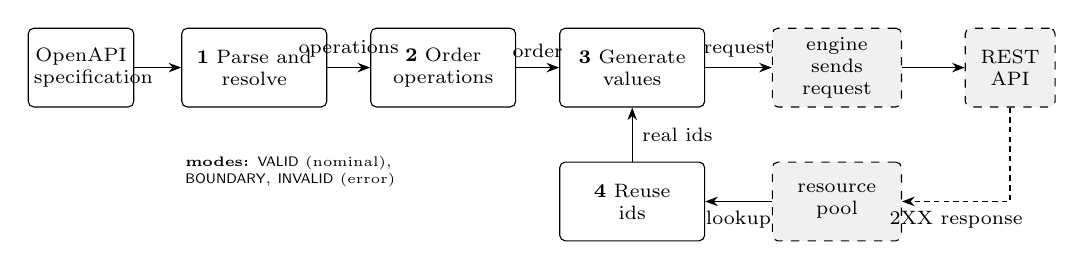
\begin{tikzpicture}[
    x=1cm, y=1cm, font=\scriptsize,
    box/.style={draw, rounded corners=2pt, align=center, inner sep=2pt,
                minimum height=10mm, text width=17mm, fill=white},
    ext/.style={draw, dashed, rounded corners=2pt, align=center, inner sep=2pt,
                minimum height=10mm, text width=15mm, fill=black!6},
    flow/.style={-{Stealth[length=1.6mm]}, line width=0.5pt},
    back/.style={-{Stealth[length=1.6mm]}, line width=0.5pt, dash pattern=on 2pt off 1.5pt},
  ]
  \node[box, text width=12mm] (spec) at (0,0) {OpenAPI\\specification};
  \node[box] (s1) at (2.2,0) {\textbf{1} Parse and\\resolve};
  \node[box] (s2) at (4.6,0) {\textbf{2} Order\\operations};
  \node[box] (s3) at (7.0,0) {\textbf{3} Generate\\values};
  \node[box] (s4) at (7.0,-1.7) {\textbf{4} Reuse\\ids};
  \node[ext] (eng) at (9.6,0) {engine\\sends request};
  \node[ext, text width=10mm] (api) at (11.8,0) {REST\\API};
  \node[ext] (pool) at (9.6,-1.7) {resource\\pool};
  \draw[flow] (spec) -- (s1);
  \draw[flow] (s1) -- node[above] {operations} (s2);
  \draw[flow] (s2) -- node[above] {order} (s3);
  \draw[flow] (s3) -- node[above] {request} (eng);
  \draw[flow] (eng) -- (api);
  \draw[back] (api.south) |- node[pos=0.75, below] {2XX response} (pool.east);
  \draw[flow] (pool) -- node[below] {lookup} (s4);
  \draw[flow] (s4) -- node[right] {real ids} (s3);
  \node[font=\tiny, align=left, anchor=north west] at (1.2,-1.0)
    {\textbf{modes:} \mode{VALID} (nominal),\\\mode{BOUNDARY}, \mode{INVALID} (error)};
\end{tikzpicture}

  \caption{Overview of \tool. Steps 1 and 2 run once per specification;
    Steps 3 and 4 run for every request. The engine and the resource pool
    (dashed, shaded) belong to the team's engine: \tool only asks the pool
    for ids. The dashed arrow is the loop that turns 2XX responses into
    real ids for later requests.}
  \label{fig:overview}
\end{figure}

\subsection{Step 1: Parse and Resolve}
\label{sec:step1}
\tool turns the specification into a list of operations whose schemas
contain no references. For each path and each HTTP method under it, it
builds one operation with (i)~its parameters; (ii)~its request body;
(iii)~one schema per response status. Five rules decide the details.
\begin{enumerate}
  \item \emph{Any reference.} A \texttt{\$ref} is a pointer into the same
    document. \tool follows it by walking the document key by key, so the
    same code resolves schemas, parameters, request bodies and responses.
  \item \emph{Recursion.} \tool passes down the set of references it is
    currently inside. When it meets one of them again, it replaces that
    reference with an empty object schema and stops. The same reference used
    twice side by side is expanded twice, because it is not a cycle.
  \item \emph{Composition.} \texttt{allOf} becomes one object schema whose
    properties and required fields are the union of its parts.
    \texttt{oneOf} and \texttt{anyOf} become their first option.
  \item \emph{Parameters.} Parameters declared on the path apply to every
    method under it; a parameter of the operation with the same name and
    location replaces them. Path parameters are always required.
  \item \emph{Base path.} If the server URL has a path, such as
    \texttt{/api/v2}, \tool puts it in front of every operation path. The
    host and port come from the test setup, not from the specification.
\end{enumerate}
We do not claim this step as new: OpenAPI libraries resolve references too.
We wrote it ourselves to keep the component free of third-party packages
inside the competition container, and we tested it with 13 small
specifications, one rule each, before running it on real ones.

\subsection{Step 2: Order Operations}
\label{sec:step2}
\tool decides which operations create the resources that others need, and
sorts the operations so that creators come first. It names every resource
with a \emph{resource key}: a lower-case word without the plural and with
\texttt{id} added, so \texttt{owners}, \texttt{ownerId} and
\texttt{owner\_id} all become \texttt{ownerid}. A bare path parameter such as
\texttt{\{id\}} takes the name of the path segment before it.

An operation \emph{produces} a key when it is a \texttt{POST} to a collection
path, such as \texttt{POST /owners}. It \emph{consumes} a key for each path
parameter, and for each required body field that names another resource,
either a field ending in \texttt{Id} or an object with an \texttt{id}
property. When no operation produces a consumed key exactly, \tool takes the
shortest producer key that ends with it or shares its first six characters,
so the body field \texttt{type} (key \texttt{typeid}) links to
\texttt{POST /pettypes} (key \texttt{pettypeid}). The \emph{depth} of an operation is the length of the
longest chain of producers before it. The final order is: creators and
readers by increasing depth, and \texttt{DELETE} operations last, deepest
first, so a pet is deleted before its owner. The idea of producer--consumer
order comes from RESTler~\cite{restler} and the operation dependency graph of
RestTestGen~\cite{resttestgen}; we use a small name-based version of it.

\subsection{Step 3: Generate Values}
\label{sec:step3}
For each request, \tool fills every required parameter, about half of the
optional ones, and the request body. It has three modes. In \mode{VALID}
mode it tries to satisfy the schema and the API. For each value it takes the
first source that applies:
(i)~an \texttt{example} or \texttt{default} in the schema;
(ii)~an \texttt{enum} member;
(iii)~a value built for the \texttt{format}, such as an ISO date for
\texttt{date} or a well-formed UUID;
(iv)~a value built for the \texttt{pattern};
(v)~a value chosen from the name, such as an e-mail address for
\texttt{email}, ten digits for \texttt{telephone}, or a small integer for a
field ending in \texttt{Id};
(vi)~a random value of the right type inside the stated limits.
For objects it leaves out read-only fields, which the server sets.

\paragraph{Patterns.} To satisfy a \texttt{pattern}, \tool parses the regular
expression with Python's own regular-expression parser and walks the parse
tree: it emits literals, picks a character from each class, and repeats each
part a random number of times inside its bounds, preferring the minimum. It
then checks the result against the pattern and the length limits, and falls
back to simpler guesses (digits only, letters only) when the check fails.

\paragraph{Error modes.} In \mode{BOUNDARY} mode, numbers and lengths sit at
their stated limits. In \mode{INVALID} mode, \tool first builds a
\mode{VALID} request and then breaks exactly one thing: one parameter, one
body field, or the whole body (a wrong type, a value outside the limits, a
missing required field, or malformed JSON). The rest of the request stays
valid, so it passes the API's first checks and the error reaches deeper
code. We do not claim error modes as new; RestTestGen also separates nominal
and error testing~\cite{resttestgen-stvr}.

\subsection{Step 4: Reuse Ids}
\label{sec:step4}
Before Step~3 builds a value for a path or query parameter, or for a body
field that looks like an id, \tool asks the resource pool for a real one:
\texttt{pool.lookup(name, schema, op)}. If the pool has one, \tool uses it.
For a body field that is itself a resource, such as the \texttt{type} of a
pet, it asks for a whole object with \texttt{pool.lookup\_object} and sends
an existing pet type. If the pool has nothing, Step~3 makes up a value. The
pool lives in the engine; \tool only reads from it.

\section{Implementation}
\label{sec:impl}

\tool is written in Python and uses only the standard library, so the
competition container needs no extra packages. It has \NLocSpec lines of
code (without blank lines and comments): \NLocParser for Step~1,
\NLocDeps for Step~2, and \NLocValues for Steps 3 and~4. The shared data
types (operation, parameter, request, response) come from the team's common
interface file and are not counted.

\paragraph{Tests.} The tests have \NLocTests lines. A ladder of \NLevels
small specifications checks Step~1 one rule at a time, from a single
\texttt{GET} up to recursive schemas, \texttt{allOf} and base paths, against
exact expected output. A second check parses all \NSpecs real specifications
and counts the operations and the references left. A third check generates
30 requests per operation and mode for every specification and fails on a
crash or on a \mode{VALID} value that breaks its schema. A fourth check uses
a stand-in pool and asserts that real ids reach the path parameters.

\paragraph{Pitfalls.} Four problems showed up only on real specifications
and APIs.
First, the flight-search specification gives some strings a
\texttt{maxLength} of $2^{31}-1$. An early version of \mode{BOUNDARY} mode
tried to build a string of that length and ran out of memory. \tool now caps
strings at 5{,}000 characters and arrays at 50 items. Second, one
specification writes its patterns in Java syntax, such as \verb|\p{L}|,
which Python cannot parse. \tool then skips its pattern generator and keeps
the values from the other sources. Third, a first live evaluation never
created a hospital on gestao-hospital. Its specification lists an
\texttt{id} field in the body of \texttt{POST /v1/hospitais/} without marking
it read-only, so \tool sent one. The API then looks for a hospital with that
\texttt{id}, finds none, and answers 400; the same body without the
\texttt{id} returns 200
(\texttt{data/diagnosis.json}). \tool now leaves out an optional field named
\texttt{id} from the body of every \texttt{POST} request. Fourth, Step~2
removes a plural \texttt{s} the English way, which turns the Portuguese
collection \texttt{hospitais} into the key \texttt{hospitaiid}, while the path
parameter \texttt{hospital\_id} becomes \texttt{hospitalid}. The two never
matched, so no hospital id was ever reused. Two keys now also match when they
share their first six characters. All results in this report come from the
version with the last two changes.

\section{Evaluation}
\label{sec:eval}

We ask four questions.
\begin{itemize}
  \item[\rqref{1}] Can \tool read the specifications that real REST APIs
    publish, including their references and composed schemas?
  \item[\rqref{2}] Do the \mode{VALID} values of \tool follow their schema
    more often than values from a simpler generator that knows only types and
    enumerations?
  \item[\rqref{3}] On running APIs, how many operations reach a 2XX response
    with each part of \tool (values, id reuse, order), and how does the
    number of unique 5XX responses change?
  \item[\rqref{4}] What does \tool cost, in time per request and in
    requests spent before the operations are reached?
\end{itemize}

\subsection{Subjects}
\label{sec:subjects}
For \rqref{1} and \rqref{2} we use all \NSpecs OpenAPI specifications that
come with the RESTgym APIs~\cite{restgym}: the ten in the RESTgym
repository and the five APIs that REST League 2027 announced for its
benchmark~\cite{restleague}. Together they have \NOpsTotal operations
(Table~\ref{tab:parser}). For \rqref{3} we need running APIs. We select
APIs with the following criteria:
\begin{enumerate}
  \item it is one of the five known REST League 2027 APIs, so the result
    matters for the competition;
  \item it runs from the released jar in a container that we can restart
    from a fresh state before every run, so runs do not affect each other;
  \item it answers requests without the authentication proxy of RESTgym, so
    our runner can talk to it directly.
\end{enumerate}
Pet-clinic (\NPetclinicOps operations, in-memory database) and
gestao-hospital (\NGestaohospitalOps operations, MongoDB) meet all three.
Flight-search expects a login token that RESTgym adds through a proxy
script, kafka-rest-proxy needs a Kafka broker, and notebook-manager needs a
MySQL server. We did not set these up in the time available.

\subsection{Baselines}
\label{sec:baselines}
We compare four configurations. Each adds one part of \tool to the previous
one, so the difference between two neighbours is the effect of that part.
\begin{description}
  \item[Baseline.] Random values that follow only the schema \texttt{type}
    and \texttt{enum}, such as eight random letters for a string, an integer
    from 0 to 1{,}000, and one item per array. This is what a simple
    schema-based random tester sends. It sees the same parsed operations as
    \tool and fills the same parameters.
  \item[+Values.] The value generator of \tool (Step~3), with no id reuse.
  \item[+Pool.] +Values, and ids reused through the resource pool (Step~4).
  \item[+Order (full).] +Pool, and the operation order of Step~2. All other
    configurations use the order of the specification file.
\end{description}
All four use the same runner, the same budget, the same seeds, and a freshly
started API. The runner and the pool are small stand-ins for the team's
engine (Section~\ref{sec:threats}), the same for every configuration.

\subsection{Measurements}
\begin{description}
  \item[\rqref{1}.] Per specification: operations found, compared with the
    method entries in the file; \texttt{\$ref} entries left after parsing;
    median parse time of five runs.
  \item[\rqref{2}.] We generate 50 \mode{VALID} requests per operation with
    each generator and fixed seeds. An \emph{input} is one sent path or query
    parameter, or one request body. An input \emph{conforms} when it
    satisfies every keyword of its schema that our checker understands:
    \texttt{type}, \texttt{enum}, \texttt{required}, \texttt{pattern},
    length and range limits, and the formats \texttt{date},
    \texttt{date-time}, \texttt{email} and \texttt{uuid}.
  \item[\rqref{3}.] Per run: $|\Reached|$ (Equation~\ref{eq:reached}) and
    $|\Faults|$ (Equation~\ref{eq:faults}). We report the mean and standard
    deviation over \NReps runs, and the union of \Faults over all runs.
  \item[\rqref{4}.] Mean time to generate one request; and the requests the
    runner spent in its nominal phase, which ends when every operation was
    either reached or tried ten times.
\end{description}

\subsection{Setup}
\label{sec:setup}
All runs used one laptop (Intel Core 7 240H, 16 logical CPUs, 8~GB of memory
for Docker, Linux 6.18 under WSL2), Python 3.14.4 and Docker 29.8.2. The APIs
ran in the \texttt{eclipse-temurin:17-jre} image from the RESTgym API
repositories at commits \texttt{e8250db} (pet-clinic) and \texttt{d4cb6c7}
(gestao-hospital); gestao-hospital used \texttt{mongo:6} with the seed data
of its repository. Every run had a budget of 20 requests per operation
(\NPetclinicBudget for pet-clinic, \NGestaohospitalBudget for
gestao-hospital). The runner first makes two nominal passes, giving each
operation up to five \mode{VALID} requests per pass until its first 2XX. The
rest of the budget goes to error requests, round-robin over the operations:
\mode{BOUNDARY} and \mode{INVALID} in turn for \tool, random values for the
baseline. Each configuration ran \NReps times, with seeds 1000 to 1004.

\subsection{\rqref{1}: Reading Real Specifications}
\label{sec:rq1}

%% Generated by src/eval/summarize.py from data/parser.csv and data/conformance.csv. Do not edit.
\begin{table}[t]
  \caption{The parser reads all 15 specifications and leaves no reference unresolved; the value generator keeps every VALID input inside its schema. \emph{Ops}: operations. \emph{\$refs}, \emph{allOf}: occurrences in the specification file. \emph{Left}: \$refs left after parsing. \emph{ms}: median parse time of five runs. \emph{Baseline}, \emph{\tool}: share of generated VALID parameter values and bodies that satisfy their schema (50 requests per operation).}
  \label{tab:parser}
  \footnotesize
  \begin{tabular}{lrrrrrrr}
    \toprule
    API & Ops & \$refs & allOf & Left & ms & Baseline & \tool \\
    \midrule
    features-service & 18 & 7 & 0 & 0 & 0.3 & 100.0\% & 100.0\% \\
    flight-search & 40 & 87 & 0 & 0 & 2.1 & 86.4\% & 100.0\% \\
    genome-nexus & 23 & 95 & 0 & 0 & 4.4 & 100.0\% & 100.0\% \\
    gestao-hospital & 20 & 25 & 0 & 0 & 0.7 & 94.3\% & 100.0\% \\
    kafka-rest-proxy & 50 & 588 & 32 & 0 & 5.1 & 98.7\% & 100.0\% \\
    languagetool & 2 & 0 & 0 & 0 & 0.1 & 100.0\% & 100.0\% \\
    market & 13 & 28 & 0 & 0 & 0.6 & 73.9\% & 100.0\% \\
    ncs & 6 & 6 & 0 & 0 & 0.7 & 100.0\% & 100.0\% \\
    notebook-manager & 5 & 6 & 0 & 0 & 0.2 & 71.4\% & 100.0\% \\
    person-controller & 12 & 16 & 0 & 0 & 0.4 & 50.0\% & 100.0\% \\
    pet-clinic & 35 & 149 & 5 & 0 & 2.8 & 80.3\% & 100.0\% \\
    project-tracking-system & 59 & 83 & 0 & 0 & 1.9 & 100.0\% & 100.0\% \\
    restcountries & 22 & 0 & 0 & 0 & 0.3 & 100.0\% & 100.0\% \\
    scs & 11 & 0 & 0 & 0 & 0.3 & 100.0\% & 100.0\% \\
    user-management & 22 & 29 & 0 & 0 & 0.8 & 88.9\% & 100.0\% \\
    \midrule
    total & 338 & 1{,}119 & 37 & 0 & & 94.2\% & 100.0\% \\
    \bottomrule
  \end{tabular}
\end{table}


Table~\ref{tab:parser} shows that \tool found every operation in every
specification and left no reference unresolved. The specifications use
references heavily: \NRefsTotal \texttt{\$ref} entries in total, and
\NRefsMax in \NRefsMaxApi alone, which also has most of the \NAllofTotal
\texttt{allOf} schemas.

\begin{observation}
\label{obs:parse}
\tool parsed all \NSpecs specifications, with \NOpsTotal operations and
\NRefsTotal references, and left \NRefsLeft references unresolved.
\end{observation}

The set has a gap. None of the \NSpecs specifications contains a recursive
schema (we counted \NRecursiveTotal), so on real data the cycle rule of
Step~1 never fired. It is covered only by the small test specifications.

\subsection{\rqref{2}: Values That Follow the Schema}
\label{sec:rq2}
The last two columns of Table~\ref{tab:parser} compare the two generators.
\tool kept \NConfTool of its \NConfToolInputs inputs inside their schema.
The baseline kept \NConfBaseline, and fell below 100\% in
\NConfBaselineBelow of the \NSpecs specifications, down to
\NConfBaselineMin for \NConfBaselineWorstApi. The baseline's \NViolBaseline
violations were almost all of two kinds that type-only generation cannot
meet: \NViolBaselineFormatPattern of them were a \texttt{format} (mostly
\texttt{date} and \texttt{date-time}) or a \texttt{pattern}.

\begin{observation}
\label{obs:conform}
\tool's \mode{VALID} inputs followed their schema in \NConfTool of cases,
against \NConfBaseline for the type-only baseline;
\NViolBaselineFormatPattern of the baseline's violations were formats or
patterns.
\end{observation}

\subsection{\rqref{3}: Operations Reached on Running APIs}
\label{sec:rq3}

%% Generated by src/eval/summarize.py from data/live/. Do not edit.
\begin{table}[t]
  \caption{Each part of \tool adds operations that reach a 2XX response. Mean over 5 runs, each on a freshly started API with the same budget of 20 requests per operation. \emph{Ops 2XX}: operations with at least one 2XX response ($\pm$ standard deviation). \emph{Share}: Ops 2XX divided by all operations. \emph{Nominal}: requests spent in the nominal phase (fewer is better). \emph{5XX}: unique 5XX responses per run. \emph{Union}: unique 5XX over all 5 runs.}
  \label{tab:live}
  \footnotesize
  \begin{tabular}{llrrrrr}
    \toprule
    API & Configuration & Ops 2XX & Share & Nominal & 5XX & Union \\
    \midrule
    \multirow{4}{*}{gestao-hospital} & Baseline & 1.0 $\pm$ 0.0 & 5.0\% & 191.0 & 1.0 $\pm$ 0.0 & 1 \\
     & +Values & 14.2 $\pm$ 1.2 & 71.0\% & 99.4 & 1.6 $\pm$ 0.5 & 2 \\
     & +Pool & 15.4 $\pm$ 0.5 & 77.0\% & 76.0 & 1.4 $\pm$ 0.5 & 2 \\
     & +Order (full) & 15.6 $\pm$ 0.5 & 78.0\% & 75.0 & 1.6 $\pm$ 0.5 & 2 \\
    \midrule
    \multirow{4}{*}{pet-clinic} & Baseline & 10.6 $\pm$ 0.8 & 30.3\% & 276.6 & 9.0 $\pm$ 0.0 & 9 \\
     & +Values & 20.0 $\pm$ 0.9 & 57.1\% & 173.8 & 83.4 $\pm$ 2.9 & 184 \\
     & +Pool & 34.0 $\pm$ 0.0 & 97.1\% & 53.2 & 98.4 $\pm$ 3.3 & 205 \\
     & +Order (full) & 33.4 $\pm$ 0.5 & 95.4\% & 52.6 & 97.8 $\pm$ 3.6 & 194 \\
    \bottomrule
  \end{tabular}
\end{table}


Table~\ref{tab:live} shows the four configurations. On pet-clinic, the
baseline reached \NPetclinicBaselineOps of \NPetclinicOps operations on
average (\NPetclinicBaselineCov). The value generator alone raised this to
\NPetclinicValuesOps (\NPetclinicValuesCov), and id reuse to
\NPetclinicValuesPlusPoolOps (\NPetclinicValuesPlusPoolCov). On
gestao-hospital, the baseline reached \NGestaohospitalBaselineOps of
\NGestaohospitalOps operations (\NGestaohospitalBaselineCov), +Values
\NGestaohospitalValuesOps (\NGestaohospitalValuesCov), and +Pool
\NGestaohospitalValuesPlusPoolOps (\NGestaohospitalValuesPlusPoolCov).

\begin{observation}
\label{obs:values}
Schema-aware values alone raised the operations reached from
\NPetclinicBaselineCov to \NPetclinicValuesCov on pet-clinic and from
\NGestaohospitalBaselineCov to \NGestaohospitalValuesCov on
gestao-hospital.
\end{observation}

\begin{observation}
\label{obs:pool}
Reusing ids from earlier responses raised the operations reached further, to
\NPetclinicValuesPlusPoolCov on pet-clinic and
\NGestaohospitalValuesPlusPoolCov on gestao-hospital.
\end{observation}

The operation order of Step~2 changed little. The full configuration reached
\NPetclinicFullOps operations on pet-clinic against
\NPetclinicValuesPlusPoolOps for +Pool, and \NGestaohospitalFullOps on
gestao-hospital against \NGestaohospitalValuesPlusPoolOps. It spent about
the same number of nominal requests (\NPetclinicFullNominal against
\NPetclinicValuesPlusPoolNominal on pet-clinic, \NGestaohospitalFullNominal
against \NGestaohospitalValuesPlusPoolNominal on gestao-hospital).
Section~\ref{sec:discussion} explains why.

\begin{observation}
\label{obs:order}
Once ids are reused, dependency order changed the operations reached by less
than one operation on average: \NPetclinicValuesPlusPoolOps to
\NPetclinicFullOps on pet-clinic and \NGestaohospitalValuesPlusPoolOps to
\NGestaohospitalFullOps on gestao-hospital.
\end{observation}

\paragraph{The motivating operation.} Over the \NReps baseline runs on
pet-clinic, the runner sent \NMotivBaselineRequests requests to
\texttt{POST /owners/\{ownerId\}/pets}. All \NMotivBaselineServer returned
500 and none created a pet. The full configuration created a pet in
\NMotivFullRunsOk of \NReps runs.

\paragraph{Unique 5XX responses.} The configurations with \tool found far
more unique 5XX responses than the baseline: \NPetclinicFullFaults per run
on pet-clinic against \NPetclinicBaselineFaults, and
\NPetclinicFullFaultsUnion against \NPetclinicBaselineFaultsUnion over all
runs. This comparison is not between equals. The baseline has no error
mode, while \tool spends the rest of its budget on \mode{BOUNDARY} and
\mode{INVALID} requests, and most of the extra 5XX responses come from them
(Section~\ref{sec:discussion}).

\begin{observation}
\label{obs:faults}
With the same budget, the full configuration produced
\NPetclinicFullFaultsUnion unique 5XX responses on pet-clinic over \NReps
runs, against \NPetclinicBaselineFaultsUnion for the baseline, and
\NGestaohospitalFullFaultsUnion against \NGestaohospitalBaselineFaultsUnion
on gestao-hospital.
\end{observation}

\subsection{\rqref{4}: Cost}
\label{sec:rq4}
Parsing took at most \NParseMsMax~ms per specification
(Table~\ref{tab:parser}). Generating one request took
\NGenUsMedian~$\mu$s at the median over the \NSpecs specifications and
\NGenUsMax~$\mu$s at most, for market, the specification with the most
\texttt{pattern} keywords. Both are small next to one
HTTP round trip to a local API. In requests, \tool makes the nominal phase
shorter, because fewer requests are rejected: on pet-clinic it fell from
\NPetclinicBaselineNominal requests for the baseline to
\NPetclinicFullNominal for the full configuration, which leaves more of the
budget for error requests.

\begin{observation}
\label{obs:cost}
\tool generated a request in \NGenUsMedian~$\mu$s at the median and cut the
nominal phase on pet-clinic from \NPetclinicBaselineNominal to
\NPetclinicFullNominal requests.
\end{observation}

\section{Discussion}
\label{sec:discussion}

\paragraph{Why does operation order add so little?} Two features of our
setup make up for a bad order. First, both APIs start with seed data: a list
request such as \texttt{GET /owners} returns existing owners and their pets,
and the pool collects their ids, so an operation can be reached before any
creator has run. Second, the runner makes two nominal passes, so an operation
that failed because its creator came later in the file gets a second try
after the creator ran. Order matters only inside the first pass, which is a
small part of the budget. An API that starts empty, or a runner that never
returns to a failed operation, would depend on order more. We leave this for
future work.

\paragraph{What does \tool still not reach?} We read the operations that
stayed unreached in the full configuration (\texttt{data/live/}).
\begin{itemize}
  \item \texttt{GET /oops} on pet-clinic returned 500 with ``No static
    resource api/oops'' to every request of every configuration. The
    operation is in the specification, but the deployed API does not serve
    it, so no input can reach a 2XX.
  \item \texttt{GET /owners/\{ownerId\}/pets/\{petId\}} on pet-clinic was
    missed in some runs. The pool picks the owner and the pet independently,
    and the API answers 404 when the pet belongs to another owner: pet~1
    returns 200 under owner~1 and 404 under owner~2
    (\texttt{data/diagnosis.json}). Picking ids that came from the same
    response should fix this.
  \item The stock operations of gestao-hospital need a
    \texttt{produto\_id} (product), but the operation that adds stock is
    named \texttt{estoque} (stock). The two words share nothing, so name
    matching cannot link them (\texttt{data/diagnosis.json} lists the keys).
  \item Patient checkout and product transfer on gestao-hospital were never
    reached. We did not find out why.
\end{itemize}
A local language model, which REST League allows, could link words such as
\texttt{estoque} and \texttt{produto}, at a far higher cost per request than
\tool has now. We leave this for future work.

\paragraph{Are the extra 5XX responses bugs?} Some are, but many are not.
On pet-clinic, a path parameter such as \texttt{ownerId=abc} returns 500
with ``Failed to convert value of type \ldots'' instead of 400. A developer
would call that a missing input check, not a crash. REST League counts each
distinct message, so the error modes of \tool raise the competition score,
but the number of unique 5XX responses overstates the number of bugs.

\section{Threats to Validity}
\label{sec:threats}

\paragraph{Internal threats.} Four things could make our comparison wrong.
First, we wrote the baseline ourselves, so it could be weaker than it should
be. Second, the live runner and the resource pool are small stand-ins that we
wrote for this evaluation, not the team's engine. Third, the same author wrote
the value generator and the schema checker of \rqref{2}, so both could share
one misreading of a keyword. Fourth, generation and the APIs are random. Our
guards:
\begin{itemize}
  \item the baseline follows the schema \texttt{type} and \texttt{enum},
    fills the same parameters as \tool, and goes through the same runner with
    the same budget; it is not tuned to fail;
  \item the runner and pool are the same for all four configurations, so the
    differences between configurations come from \tool;
  \item the checker parses dates and UUIDs with Python's standard library, not
    with code from \tool, and \rqref{2} counts only keywords that the checker
    understands;
  \item every configuration ran \NReps times with fixed seeds, each time on a
    freshly started API, and Table~\ref{tab:live} reports the standard
    deviation.
\end{itemize}
What remains: a real engine chooses requests from feedback, and may narrow or
widen the gaps we measured. Our 5XX signature masks quoted text in error
messages; two faults that differ only in a quoted name count as one, so
\Faults may be smaller than the number of distinct messages. In a trial run
we read the signatures of the operation with the most 5XX responses and found
no duplicates caused by echoed input.

\paragraph{External threats.} We ran \tool live on two APIs, both written in
Java with Spring, out of the five known REST League APIs, and the competition
adds five APIs that nobody has seen. All \NSpecs specifications are
OpenAPI~3.0 files in JSON. \tool reads YAML only when the PyYAML package is
present and does not read Swagger~2.0 at all, so an unseen API with such a
specification would fail at Step~1. None of the specifications had a
recursive schema. We used one machine and one version of each tool, listed in
Section~\ref{sec:setup}.

\paragraph{Construct threats.} We measure what REST League scores, but the
scores are proxies. An operation counts as reached after one 2XX response,
even when that response did little, such as a list request on an empty
collection. A unique 5XX response is not always a bug that a developer would
fix: many of the 5XX responses we saw on pet-clinic are wrong parameter types
that the API reports as 500 instead of 400. They count in the competition, so
we count them, but we do not call them bugs. Schema conformance in \rqref{2}
means only that a value fits the schema; the API can still reject it, which
is why \rqref{3} measures acceptance on running APIs. We did not measure code
coverage, the third REST League metric, because our runner talks to the APIs
directly instead of through RESTgym's coverage collection.
         % or merge into discussion to save space
\section{Related Work}
\label{sec:related}

\paragraph{Realistic input values.} Closest to us is work that makes REST
inputs look like real data. ARTE~\cite{arte} finds realistic values for
parameters by querying a public knowledge base with the parameter's name and
description. NLP2REST~\cite{nlp2rest} reads the natural-language descriptions
in a specification and turns them into extra rules, such as value ranges and
formats, that tools can use. We share their goal of getting past input
validation, but \tool uses only what the schema states (formats, patterns,
limits, examples) and the parameter names, with no network access and no
language model. This fits the REST League sandbox, which allows no remote
services, and it costs microseconds per request. The price is that \tool
cannot invent a meaningful free-text value, such as a real city for a
parameter called \texttt{location}.

\paragraph{Operation dependencies.} RESTler~\cite{restler} infers
producer--consumer relations from the specification and uses the ids in
responses to build sequences of requests. RestTestGen~\cite{resttestgen}
builds an operation dependency graph from matching field names and tests
operations in its order. Morest~\cite{morest} keeps a property graph that it
updates with what it learns during the run. ARAT-RL~\cite{arat-rl} uses
reinforcement learning to decide which operations and parameters to try and
reuses values seen in responses. Martin-Lopez et al.\ go one level deeper and
model the constraints between parameters of the same
operation~\cite{idl}. We use a deliberately small version of
producer--consumer order. What we add is a measurement of how much order
contributes once ids are already reused: on the APIs we tested, less than one
operation (Observation~\ref{obs:order}).

\paragraph{Complete testing tools.} EvoMaster~\cite{evomaster} generates
tests with an evolutionary search guided by code coverage, which needs access
to the code.
Schemathesis~\cite{schemathesis} derives property-based tests from the
schema. RESTest~\cite{restest} generates tests from a specification extended
with inter-parameter constraints. DeepREST~\cite{deeprest} learns a testing
policy with deep reinforcement learning. RestTestGen separates nominal and
error testing~\cite{resttestgen-stvr}, which our \mode{VALID} and
\mode{INVALID} modes follow. All of these are complete tools with their own
input generators. \tool is one component of a tool, and we evaluate it on
its own, with the other parts held fixed, so that its effect is not mixed
with that of a search strategy.

\paragraph{Empirical comparisons.} Corradini et al.\ compared black-box
REST testing tools on the same APIs~\cite{corradini-comparison}. Kim et
al.\ compared tools on real-world services and listed open problems for the
field, among them producing valid input values and handling dependencies
between operations~\cite{no-time-to-rest}. RESTgym~\cite{restgym} and REST
League~\cite{restleague} provide the shared infrastructure and scoring that
we follow. Their studies compare complete tools; we compare configurations of
one component on the same runner, which shows which part of the input side
moves the score.

\section{Conclusion}
\label{sec:conclusion}

A black-box REST API tester can only test what its requests reach. When it
follows only the types in the specification, the API rejects most of its
requests at the first check: on pet-clinic, a type-only generator reached
\NPetclinicBaselineCov of the operations, and all \NMotivBaselineRequests of
its requests to add a pet failed while parsing a random date.

We presented \tool, which parses an OpenAPI specification, generates values
from examples, formats, patterns and names, reuses real ids from earlier
responses, and orders operations by their dependencies. It parsed all
\NSpecs specifications we tried. It kept \NConfTool of its generated values
inside their schema, against \NConfBaseline for a type-only generator. It
raised the operations reached from \NPetclinicBaselineCov to
\NPetclinicFullCov on pet-clinic and from \NGestaohospitalBaselineCov to
\NGestaohospitalFullCov on gestao-hospital with the same request budget.
Values and id reuse gave this gain; operation order changed it by less than
one operation.

\section*{Data Availability}
\label{sec:data}
The replication package is the submission repository itself. Its
\texttt{src/} folder contains the source of \tool with its tests, the
\NSpecs specifications we used, the evaluation scripts, and a script that
fetches the two APIs at the exact commits we tested. Its
\texttt{paper/data/} folder contains every raw result: one JSON file per live
run with per-operation counts and every 5XX signature, the CSV files of the
offline evaluation, and the file of numbers that this paper prints.
\texttt{src/README.md} lists the commands that regenerate each file.

\section*{Use of Generative AI}
A generative AI assistant (Claude Opus 5.5, by Anthropic) was used in this
project. It wrote most of the source code of \tool and of the evaluation
scripts from the author's task description and the team's interface file,
helped find and fix defects found by the tests, looked up and checked the
bibliographic data of the cited papers against Crossref, and drafted the
text of this report. The author reviewed the code, the text and the
citations. All numbers reported here were produced by running the tool and
scripts in \texttt{src/}; the paper reads them from a generated file.


\bibliographystyle{ACM-Reference-Format}
\bibliography{references}

\end{document}
